\documentclass[12pt,reqno]{article}

%%%%%%%%%%%%%%%%%%%% PACKAGES %%%%%%%%%%%%%%%%%%%%

\usepackage[utf8]{inputenc}
\usepackage[all]{xy}
\usepackage[T1]{fontenc}
\usepackage[usenames, dvipsnames]{color}
\usepackage{setspace}
\usepackage{dsfont}
\usepackage{amssymb}
\usepackage{amsthm,bbm}
\usepackage{amscd}
\usepackage{amsfonts}
\usepackage{stmaryrd}
\usepackage{amsmath}
\usepackage{graphicx}
\usepackage{multicol}
\usepackage{xspace}
\usepackage{extarrows}
\usepackage{color}
\usepackage [english]{babel}
\usepackage [autostyle, english = american]{csquotes}
\usepackage[colorlinks, linktocpage, citecolor = red, linkcolor = blue]{hyperref}
\usepackage{fullpage}
\usepackage{color}
\usepackage{euler}
\usepackage{parskip}
\usepackage{tikz}

%%%%%%%%%%%%%%%%%%%% INITIALIZATION %%%%%%%%%%%%%%%%%%%%

\MakeOuterQuote{"}
\graphicspath{ {./} }

%%%%%%%%%%%%%%%%%%%% COMMANDS %%%%%%%%%%%%%%%%%%%%

\newcommand{\range}{\mathrm{range\,}}
\newcommand{\nul}{\mathrm{null\,}}
\newcommand{\spn}{\mathrm{span\,}}
\newcommand{\card}{\mathrm{cardinality}}
\newcommand{\R}{\mathbb{R}}
\newcommand{\C}{\mathbb{C}}
\newcommand{\F}{\mathbb{F}}
\newcommand{\Z}{\mathbb{Z}}
\newcommand{\bd}{\mathrm{bd\,}}
\newcommand{\divline}{\hrule\vspace{12pt}\noindent}
\newcommand{\sgn}{\mathrm{sgn}}

%%%%%%%%%%%%%%%%%%%% ENVIRONMENTS %%%%%%%%%%%%%%%%%%%%

\theoremstyle{plain}
\newtheorem{maintheorem}{Theorem}
\renewcommand*{\themaintheorem}{\Alph{maintheorem}}

\newtheorem{theorem}{Theorem}[section] 
\newtheorem{lemma}{Lemma}
\newtheorem{corollary}[theorem]{Corollary}

\theoremstyle{definition}
\newtheorem{problem}{Problem}
\newtheorem{example}[theorem]{Example}
\newtheorem{definition}[theorem]{Definition}
\newtheorem{question}[theorem]{Question}

\newtheorem*{maintheorema}{Theorem \ref{thm:main}}

%%%%%%%%%%%%%%%%%%%% TITLE-PAGE %%%%%%%%%%%%%%%%%%%%

\title{MATH 1530 Problem Set 5}
\author{Tanish Makadia\\\small{(Collaborated with Esmé and Kazuya)}}
\date{March 2023}

%%%%%%%%%%%%%%%%%%%% DOCUMENT %%%%%%%%%%%%%%%%%%%%

\begin{document}
\maketitle

%%%%%%%%%%%%%%%%%%%% PROBLEM 1 %%%%%%%%%%%%%%%%%%%%

\begin{problem} 
    How many elements of order 6 are in $S_7$?
\end{problem}

\begin{proof}
    By (Gallian, 5.1), every permutation of a finite set can be expressed as a product of
    disjoint cycles. Additionally, by (Gallian, 5.3), the order of a permutation in disjoint
    cycle form is the \(lcm\) of lengths of the disjoint cycles.
     
    Let \(P = \{s\in S_7\ |\ |s|=6\}\). We must find the cardinality of \(P\). Let \(p\in P\). From above, \(p\) must have a disjoint cycle form in which the \(lcm\) of
    the disjoint cycle lengths equals \(6\). Therefore, the disjoint cycle form of \(p\) must fall under one
    of the following cases: (note that the order of the disjoint cycles does not matter since they are commutative)
    \begin{itemize}
        \item \textbf{Case 1 (lengths: \(3, 2, 2\)):} \(p = (a_1, a_2)(b_1, b_2)(c_1, c_2, c_3)\). In this case, the number of ways to construct \(p\) using
        elements of \(S_7\) is:
        \[\binom{7}{3}\frac{3!}{3}\cdot\binom{4}{2}\frac{2!}{2}\cdot\binom{2}{2}\frac{2!}{2}\cdot \frac{1}{2}=210\]
        Essentially, each \(\binom{n}{k}\) is the number of unique combinations of elements for a single cycle of length \(k\). We multiply this by
        \(\frac{k!}{k}\) in order to account for all the unique orderings of elements within that cycle.
        In this case, we must also divide by \(2\) since the order of either two-cycle does not matter.
        \item \textbf{Case 2 (lengths: \(3,2,1,1\)):} \(p = (a_1,a_2,a_3)(b_1,b_2)(c_1)(d_1)\). In this case, the number of ways to construct
        \(p\) is:
        \[\binom{7}{3}\frac{3!}{3}\cdot\binom{4}{2}\frac{2!}{2}=420\]
        \item \textbf{Case 3 (lengths: \(6,1\)):} \(p=(a_1,a_2,a_3,a_4,a_5,a_6)(b_1)\). In this case, the number of ways to construct
        \(p\) is:
        \[\binom{7}{6}\frac{6!}{6}=840\]
    \end{itemize}
    Therefore, the number of elements of order \(6\) in \(S_7\) is \(\mathrm{card}(P)=210+420+840=1470\).
\end{proof}

\newpage

%%%%%%%%%%%%%%%%%%%% PROBLEM 2 %%%%%%%%%%%%%%%%%%%%

\begin{problem} 
    Let $D_4$ denote the rigid operations on a square taking the square back to itself (i.e., the symmetries of the square). For example, rotating the square by $\pi$ is a rigid operation taking the square back to itself. This is called the \emph{dihedral group}, and it is a group under composition.
    
    Label the vertices of the square from 1 to 4. Use this to represent the elements of $D_4$ a subgroup of $S_4$ (that is, list the elements of $D_4$ using cycle notation). What is the order of $D_4?$ Is $D_4$ isomorphic to $S_4$?
\end{problem}

\begin{proof} The elements of \(D_4\) are the following permutations in \(S_4\):
    \begin{align*}
        &\begin{tikzpicture}
            \draw (0,0) -- (0,1.5) -- (1.5,1.5) -- (1.5,0) -- (0,0);
            \node at (-1, 0.75) {1.};
            \node[above right] at (0,0) {4};
            \node[below right] at (0,1.5) {1};
            \node[below left] at (1.5,1.5) {2};
            \node[above left] at (1.5,0) {3};
            \node at (5,0.75) {\(\xrightarrow[e]{\text{identity}}\)};
        \end{tikzpicture}
        &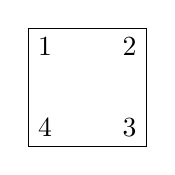
\begin{tikzpicture}
            \draw (0,0) -- (0,1.5) -- (1.5,1.5) -- (1.5,0) -- (0,0);
            \node[below right] at (0,1.5) {1};
            \node[below left] at (1.5,1.5) {2};
            \node[above left] at (1.5,0) {3};
            \node[above right] at (0,0) {4};
        \end{tikzpicture}
        \\
        &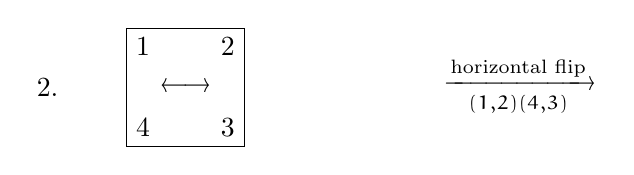
\begin{tikzpicture}
            \draw (0,0) -- (0,1.5) -- (1.5,1.5) -- (1.5,0) -- (0,0);
            \node at (-1, 0.75) {2.};
            \node[below right] at (0,1.5) {1};
            \node[below left] at (1.5,1.5) {2};
            \node[above left] at (1.5,0) {3};
            \node[above right] at (0,0) {4};
            \node at (0.75,0.75) {\(\longleftrightarrow\)};
            \node at (5,0.75) {\(\xrightarrow[(1,2)(4,3)]{\text{horizontal flip}}\)};
        \end{tikzpicture}
        &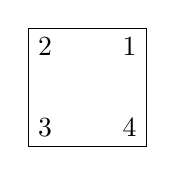
\begin{tikzpicture}
            \draw (0,0) -- (0,1.5) -- (1.5,1.5) -- (1.5,0) -- (0,0);
            \node[below right] at (0,1.5) {2};
            \node[below left] at (1.5,1.5) {1};
            \node[above left] at (1.5,0) {4};
            \node[above right] at (0,0) {3};
        \end{tikzpicture}
        \\
        &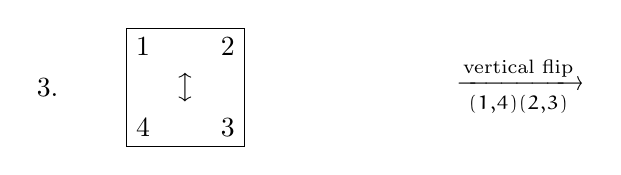
\begin{tikzpicture}
            \draw (0,0) -- (0,1.5) -- (1.5,1.5) -- (1.5,0) -- (0,0);
            \node at (-1, 0.75) {3.};
            \node[below right] at (0,1.5) {1};
            \node[below left] at (1.5,1.5) {2};
            \node[above left] at (1.5,0) {3};
            \node[above right] at (0,0) {4};
            \node at (0.75,0.75) {\(\updownarrow\)};
            \node at (5,0.75) {\(\xrightarrow[(1,4)(2,3)]{\text{vertical flip}}\)};
        \end{tikzpicture}
        &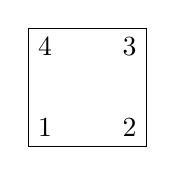
\begin{tikzpicture}
            \draw (0,0) -- (0,1.5) -- (1.5,1.5) -- (1.5,0) -- (0,0);
            \node[below right] at (0,1.5) {4};
            \node[below left] at (1.5,1.5) {3};
            \node[above left] at (1.5,0) {2};
            \node[above right] at (0,0) {1};
        \end{tikzpicture}
        \\
        &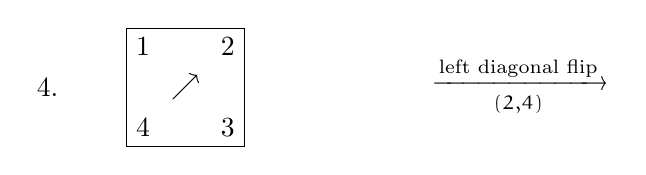
\begin{tikzpicture}
            \draw (0,0) -- (0,1.5) -- (1.5,1.5) -- (1.5,0) -- (0,0);
            \node at (-1, 0.75) {4.};
            \node[below right] at (0,1.5) {1};
            \node[below left] at (1.5,1.5) {2};
            \node[above left] at (1.5,0) {3};
            \node[above right] at (0,0) {4};
            \node at (0.75,0.75) {\(\nearrow\)};
            \node at (5,0.75) {\(\xrightarrow[(2,4)]{\text{left diagonal flip}}\)};
        \end{tikzpicture}
        &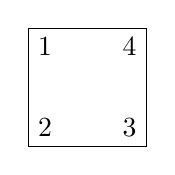
\begin{tikzpicture}
            \draw (0,0) -- (0,1.5) -- (1.5,1.5) -- (1.5,0) -- (0,0);
            \node[below right] at (0,1.5) {1};
            \node[below left] at (1.5,1.5) {4};
            \node[above left] at (1.5,0) {3};
            \node[above right] at (0,0) {2};
        \end{tikzpicture}
        \\
        &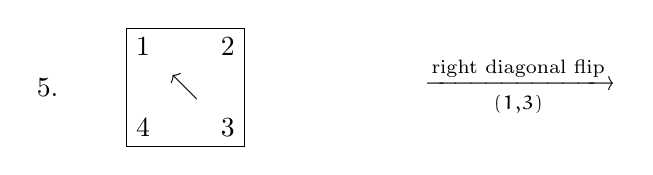
\begin{tikzpicture}
            \draw (0,0) -- (0,1.5) -- (1.5,1.5) -- (1.5,0) -- (0,0);
            \node at (-1, 0.75) {5.};
            \node[below right] at (0,1.5) {1};
            \node[below left] at (1.5,1.5) {2};
            \node[above left] at (1.5,0) {3};
            \node[above right] at (0,0) {4};
            \node at (0.75,0.75) {\(\nwarrow\)};
            \node at (5,0.75) {\(\xrightarrow[(1,3)]{\text{right diagonal flip}}\)};
        \end{tikzpicture}
        &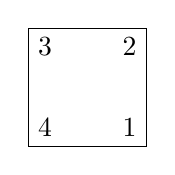
\begin{tikzpicture}
            \draw (0,0) -- (0,1.5) -- (1.5,1.5) -- (1.5,0) -- (0,0);
            \node[below right] at (0,1.5) {3};
            \node[below left] at (1.5,1.5) {2};
            \node[above left] at (1.5,0) {1};
            \node[above right] at (0,0) {4};
        \end{tikzpicture}
        \\
        &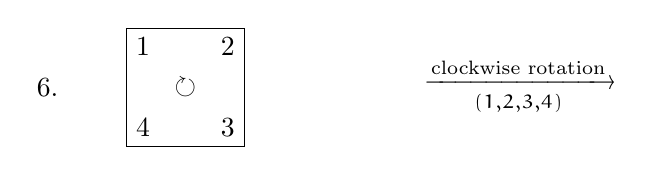
\begin{tikzpicture}
            \draw (0,0) -- (0,1.5) -- (1.5,1.5) -- (1.5,0) -- (0,0);
            \node at (-1, 0.75) {6.};
            \node[below right] at (0,1.5) {1};
            \node[below left] at (1.5,1.5) {2};
            \node[above left] at (1.5,0) {3};
            \node[above right] at (0,0) {4};
            \node at (0.75,0.75) {\(\circlearrowright\)};
            \node at (5,0.75) {\(\xrightarrow[(1,2,3,4)]{\text{clockwise rotation}}\)};
        \end{tikzpicture}
        &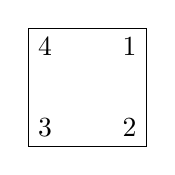
\begin{tikzpicture}
            \draw (0,0) -- (0,1.5) -- (1.5,1.5) -- (1.5,0) -- (0,0);
            \node[below right] at (0,1.5) {4};
            \node[below left] at (1.5,1.5) {1};
            \node[above left] at (1.5,0) {2};
            \node[above right] at (0,0) {3};
        \end{tikzpicture}
        \\
        &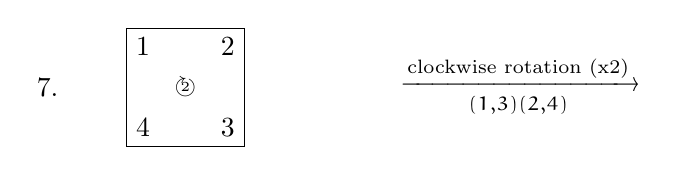
\begin{tikzpicture}
            \draw (0,0) -- (0,1.5) -- (1.5,1.5) -- (1.5,0) -- (0,0);
            \node at (-1, 0.75) {7.};
            \node[below right] at (0,1.5) {1};
            \node[below left] at (1.5,1.5) {2};
            \node[above left] at (1.5,0) {3};
            \node[above right] at (0,0) {4};
            \node at (0.75,0.75) {\(\circlearrowright\)};
            \node at (0.75,0.75) {\tiny{2}};
            \node at (5,0.75) {\(\xrightarrow[(1,3)(2,4)]{\text{clockwise rotation (x2)}}\)};
        \end{tikzpicture}
        &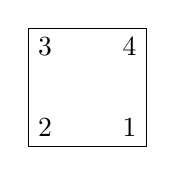
\begin{tikzpicture}
            \draw (0,0) -- (0,1.5) -- (1.5,1.5) -- (1.5,0) -- (0,0);
            \node[below right] at (0,1.5) {3};
            \node[below left] at (1.5,1.5) {4};
            \node[above left] at (1.5,0) {1};
            \node[above right] at (0,0) {2};
        \end{tikzpicture}
        \\
        &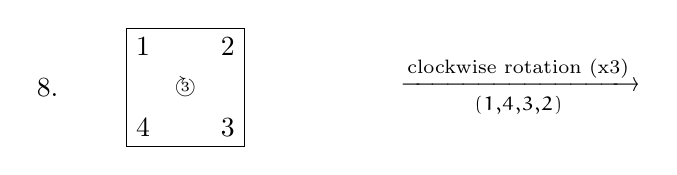
\begin{tikzpicture}
            \draw (0,0) -- (0,1.5) -- (1.5,1.5) -- (1.5,0) -- (0,0);
            \node at (-1, 0.75) {8.};
            \node[below right] at (0,1.5) {1};
            \node[below left] at (1.5,1.5) {2};
            \node[above left] at (1.5,0) {3};
            \node[above right] at (0,0) {4};
            \node at (0.75,0.75) {\(\circlearrowright\)};
            \node at (0.75,0.75) {\tiny{3}};
            \node at (5,0.75) {\(\xrightarrow[(1,4,3,2)]{\text{clockwise rotation (x3)}}\)};
        \end{tikzpicture}
        &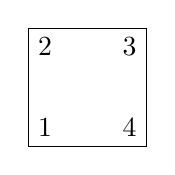
\begin{tikzpicture}
            \draw (0,0) -- (0,1.5) -- (1.5,1.5) -- (1.5,0) -- (0,0);
            \node[below right] at (0,1.5) {2};
            \node[below left] at (1.5,1.5) {3};
            \node[above left] at (1.5,0) {4};
            \node[above right] at (0,0) {1};
        \end{tikzpicture}
    \end{align*}
    Evidently, \(|D_4|=8\). Since \(|S_4|=4!=24\neq 8\), by (Gallian, 6.2.7), we have that \(D_4\not\approx S_4\).
\end{proof}

\newpage

%%%%%%%%%%%%%%%%%%%% PROBLEM 3 %%%%%%%%%%%%%%%%%%%%

\begin{problem}  
    Prove that a permutation with odd order must be an even permutation. Show that the converse is false.
\end{problem}

\begin{proof}
    Let \(p\) be a permutation such that \(|p|=n\) where \(n\) is odd. We have that, \(p^n=e\).
    By (Gallian, 5.4), \(p=\beta_1\cdots\beta_r\) where each \(\beta_i\) is a two-cycle.
    Combining these two equations, we obtain \((\beta_1\cdots\beta_r)^n=e\). For contradiction,
    suppose \(r\) is odd. Thus, we have that
    \begin{align*}
        e &= (\beta_1\cdots\beta_r)^n\\
        &= (\beta_1\cdots\beta_r)\ \overset{n\text{ times}}{\cdots}\ (\beta_1\cdots\beta_r)\\
        &= \beta_1\cdots\beta_{nr}
    \end{align*}
    By lemma \ref{lem:oddmult}, \(nr\) is odd. Since \(e\) must equal the product of an even number of two cycles, this is a contradiction.
    Therefore, \(r\) must be even which implies that \(p\) is an even permutation.
\end{proof}
\bigskip
\begin{proof}
    We will provide a counter-example to show that an even permutation is not necessarily of odd order.
    Consider the even permutation \((1,2)(3,4)\). Evidently, \(((1,2)(3,4))^2=(1,2)(3,4)(1,2)(3,4)=(1)(2)(3)(4)=e\). This implies that
    \((1,2)(3,4)\) is of even order.
\end{proof}
\bigskip
\begin{lemma}
    \label{lem:oddmult}
    The product of two odd integers is odd
    \begin{proof}
        Let \(x,y\in\Z\) such that \(x\) and \(y\) are odd. By the division algorithm, we have that
        \(x=2b_x+1\) and \(y=2b_y+1\) where \(b_x,b_y\in\Z\). Now consider the product of \(x\) and \(y\):
        \begin{align*}
            x\cdot y &= (2b_x+1)\cdot (2b_y+1)\\
            &= 4b_xb_y+2b_x+2b_y+1\\
            &= 2(2b_xb_y+b_x+b_y)+1
        \end{align*}
        Therefore, \(2\nmid x\cdot y\implies x\cdot y\) is odd.
    \end{proof}
\end{lemma}

\newpage

%%%%%%%%%%%%%%%%%%%% PROBLEM 4 %%%%%%%%%%%%%%%%%%%%

\begin{problem} 
    Let $\mathbb{C}$ be the complex numbers and 
    $$
    M = \left \{
    \begin{bmatrix}
       a  & -b \\
       b  &  a
    \end{bmatrix}
    \middle| \  a,b \in \mathbb{R}
    \right \}.
    $$
    prove that $\mathbb{C}^*$ and $M^*$ (the nonzero elements of $M$), viewed as groups with multiplication, are isomorphic. 
\end{problem}

\begin{proof}
    We will prove that the following function is an isomorphism from \(\C^*\) to \(M^*\):
    \begin{align*}
        \phi:\C^*&\to M^*\\
        a+bi&\mapsto \begin{bmatrix}
            a & -b\\
            b & a
        \end{bmatrix}
    \end{align*} 
    \begin{itemize}
        \item \textbf{Injective: } Let \(u,v\in\C^*\) such that \(u=a+bi\) and \(v=c+di\) where \(a,b,c,d\in\R\).
        \(\phi(u)=\phi(v)\implies
            \begin{bmatrix}
                a & -b\\
                b & a
            \end{bmatrix}
            =
            \begin{bmatrix}
                c & -d\\
                d & c
            \end{bmatrix}
        \implies a=c\text{ and }b=d\implies u=v\).
        \item \textbf{Surjective: }
        \begin{align*}
            \range(\phi) &= \{\phi(u)\ |\ u\in\C^*\}\\
            &= \{\phi(a+bi)\ |\ a,b\in\R\}\\
            &= 
            \biggl\{
                \begin{bmatrix}
                    a & -b\\
                    b & a
                \end{bmatrix}
                \ \bigg|\ a,b\in\R
            \biggr\}\\
            &= M^*
        \end{align*}
    \item \textbf{Preserves Group Operation: } Let \(u,v\in\C^*\) such that \(u=a+bi\) and \(v=c+di\) where \(a,b,c,d\in\R\).
    \begin{align*}
        \phi(u\cdot v) &= \phi((a+bi)\cdot (c+di))\\
        &= \phi(ac+adi+bci+bdi^2)\\
        &= \phi((ac-bd)+(ad+bc)i)\\
        &= \begin{bmatrix}
            ac-bd & -ad-bc\\
            ad+bc & ac-bd
        \end{bmatrix}\\
        &= \begin{bmatrix}
            a & -b\\
            b & a
        \end{bmatrix}
        \begin{bmatrix}
            c & -d\\
            d & c
        \end{bmatrix}\\
        &= \phi(u)\cdot\phi(v)
    \end{align*}
    \end{itemize}
    Therefore, we have proven that \(\C^*\) and \(M^*\) are isomorphic.
\end{proof}

\newpage

%%%%%%%%%%%%%%%%%%%% PROBLEM 5 %%%%%%%%%%%%%%%%%%%%

\begin{problem} Let $G$ be a group. An isomorphism from $G$ to itself is called an \emph{automorphism} of $G$. Let $\mathrm{Aut}(G)$ denote the set of all automorphisms of $G$. This is a group under the operation of function composition.
    Find two groups $G$ and $H$ such that $G \not \approx H$ but $\mathrm{Aut}(G) \approx \mathrm{Aut}(H)$.
\end{problem}

\begin{proof}
    Let \(G=(\Z, +)\) and let \(H=\Z_4\). We will now determine \(Aut(G)\) and \(Aut(H)\).
    \begin{itemize}
        \item \underline{\(Aut(G)\)}: Let \(k\in G\) and let \(\alpha\in Aut(G)\). We have that
        \begin{align*}
            \alpha(k)&=\alpha(1+\ \overset{k\text{ times}}{\cdots}\ +1)\\
            &=\alpha(1)+\ \overset{k\text{ times}}{\cdots}\ +\alpha(1)\\
            &=k\alpha(1)
        \end{align*}
        Therefore, the number of distinct automorphisms
        in \(Aut(G)\) is equal to the number of distinct elements that \(1\) can be mapped to.
        Since \[(\Z,+)=\{1^n\ |\ n\in\Z\}=\{(-1)^n\ |\ n\in\Z\}\]
        we have that \(G=\langle 1\rangle=\langle -1\rangle\). Since \(1\) is a generator of \(G\), by (Gallian, 6.2.4) it must be the case
        that \(\langle\alpha(1)\rangle\) is also a generator of \(G\). Thus, \(\alpha(1)=1\text{ or }-1\). Let \(\alpha_1,\alpha_{-1}\in Aut(G)\)
        denote the automorphisms that map \(1\) to \(1\) and \(-1\) respectively. Therefore, we have that
        \(Aut(G)=\{\alpha_1,\alpha_{-1}\}\).

        \item \underline{\(Aut(H)\)}: Let \(\overline{\alpha}\in Aut(H)\). A similar process can be used to show that the number of distinct automorphisms
        in \(Aut(H)\) is equal to the number of distinct elements that \(1\) can be mapped to. Since
        \[H=\{0,1,2,3\}\qquad\text{ and }\qquad |1|=4\]
        we have that \(|\overline{\alpha}(1)|=4\). Hence, \(\overline{\alpha}(1)=1\text{ or }3\). Let \(\overline{\alpha}_1,\overline{\alpha}_3\in Aut(H)\)
        denote the automorphisms that map \(1\) to \(1\) and \(3\) respectively.
        Therefore, we have that \(Aut(H)=\{\overline{\alpha}_1,\overline{\alpha}_3\}\).
    \end{itemize}

    Evidently, \(G\not\approx H\) since \(|G|\neq|H|\). Additionally, \(|Aut(G)|=|Aut(H)|=2\). Since there is only one way
    to construct a group of order \(2\) (using an identity and an element that is its own inverse), it must be the case that
    \(Aut(G)\approx Aut(H)\).
\end{proof}

\end{document}